\documentclass{article}
\usepackage[margin=1.5cm]{geometry}
\usepackage{microtype} % Slightly better kerning
\usepackage{graphicx}
\graphicspath{ {./figs/} }
\usepackage[colorlinks=true]{hyperref}
\setlength{\parindent}{0pt}
\setlength{\parskip}{1em}
\usepackage{fancyhdr} % Needed to adjust page numbering
\usepackage{lastpage} % Counts total number of pages

\pagestyle{fancy}
\fancyhf{}
\renewcommand{\headrulewidth}{0pt} % Remove header line
\cfoot{\thepage \hspace{1pt} of \pageref*{LastPage}} % Customize page nums


\usepackage{amsmath}
\usepackage{upgreek}

\usepackage{array} % New env. for equation conditions where aligned
\newenvironment{conditions}[1][where:] 
  {#1 \begin{tabular}[t]{>{$}l<{$} @{${}={}$} l}}
  {\end{tabular}\\[\belowdisplayskip]}

\title{Spatial Interpolation Notes}

\begin{document}
\maketitle

\section{Introduction}

We want to use interpolation because it is reasonable to assume that spatially distributed variables are also spatially correlated.
It is not always true, but often worth exploring as part of an analysis.
There are multiple different methods to interpolate data that depend on different underlying assumptions.
These methods are described below.

\begin{center}
    \fbox{Information from \href{https://desktop.arcgis.com/en/arcmap/10.3/tools/3d-analyst-toolbox/how-kriging-works.htm}{ARCGIS} and Applied Spatial Data Analysis With R (2013) unless listed otherwise}
\end{center}

There are two main methods used to interpolate data and estimate a surface for geospatial data:

\begin{itemize}
    \item Inverse distance weighting (IDW) and spline methods
    \item Kriging
\end{itemize}

IDW and splines are deterministic interpolation methods as they are directly based on the surrounding values or smoothed formulas.
Kriging is different as it uses autocorrelation and takes position into account in the statistical models.
Kriging uses a certain number of neighbouring points, or all points within a specified radius (cf kNN).

The general formula for IDW and kriging is:

\[\hat{Z}(s_{0} )=\sum_{i=1}^{N} w(s_{i}) Z (s_{i})\]

\begin{conditions}
Z(s_{i}) & the measured value at the $i$th location \\
w(s_{i}) & an unknown weight for the measured value at the $i$th location \\
s_{0} & the prediction location \\
N & the number of measured values
\end{conditions}

The difference between IDW and kriging is that in IDW, $w(s_{i})$ only depends on distance to prediction location.
In kriging $w(s_{i})$ also depends on autocorrelation i.e. spatial relationship between prediction locations.

\section{Inverse distance weighting (IDW)}

IDW determines cell values using a linearly weighted combination of surrounding values.
The weights are function of the inverse distance.
The general form for the IDW function is:

\[\hat{Z}(s_{0})= \frac{\sum_{i=1}^{n} w(s_{i}) Z(s_{i})}{\sum_{i=1}^{n} w (s_{i})}\]

\begin{conditions}
    Z(s_{i}) & the measured value at the $i$th location \\
    w(s_{i}) & $||s_{i} - s_{0}||^{-p}$ \\
    || \cdot || & Euclidean distance \\
    p & an inverse distance weighting power, defaulting to 2
\end{conditions}

The value of $p$ determines how much closer values are preferred.
As $p$ increases, IDW approaches a one-nearest-neighbour interpolation model.
$p$ can be selected using cross-validation.

Another way to control IDW interpolation is through selecting the number of neighbouring observations to include.
This can improve speed of interpolation, and may be used when there is reason to believe that distant points have little correlation.
There are two approaches for varying the number of points used for interpolation:

\begin{enumerate}
    \item Varying search radius 
    \begin{itemize}
        \item The number of points to include is fixed, and the radius changes to include that set number
        \item Depends on the density of observations fluctuating
        \item The maximum radius can also be set, in which case all points will be included if that max radius is reached before $n$
    \end{itemize}
    \item Fixed search radius
    \begin{itemize}
        \item Set a radius and minimum number of points
        \item If $n <$ minimum number of points at set radius, the radius increases until the minimum is reached.
    \end{itemize}
\end{enumerate}

In addition to these two approaches, barriers can be created to limit the searches for neighbouring points, i.e. only search for this side of a river.

\section{Kriging}

One of the key benefits of kriging is that in addition to using autocorrelation, it is able to estimate uncertainty in the interpolation.
It can do this because it is based on a spatial arrangement of empirical observations, rather than a presumed model of spatial distribution.
Although kriging preferentially weights closer observations, its use of autocorrelation means that clusters are not over-fit i.e. lowering bias as each point in a cluster provides less information than a single point.

The kriging predictor is an "optimal linear predictor" and an exact interpolator.
This means that prediction error is each interpolated value is calculated to minimize the prediction error for that point.
It also means that the interpolated value for sampled points is equal to the actual value, and all interpolated values will be the Best Linear Unbiased Predictors (BLUPs).

Kriging is only helpful where there is at least moderate spatial autocorrelation.
If there is not, then simpler methods like IDW, will generally perform as well as kriging.

\subsection{Assumptions in kriging}

\begin{center}
    \fbox{Information for assumptions from \href{https://www.publichealth.columbia.edu/research/population-health-methods/kriging-interpolation}{Columbia}}    
\end{center}

For kriging to be used, there are a number of assumptions/conditions to be met.
These conditions can be checked in exploratory data analysis.

\begin{enumerate}
    \item Assumption of intrinsic stationarity
    \begin{itemize}
        \item Means that the joint probability distribution does not vary across the study space, so the same parameters (e.g. mean, range and sill etc) are valid across the space
        \item Means one variogram is valid across the space
    \end{itemize}
    \item Assumption of isotropy
    \begin{itemize}
        \item Uniformity in all directions (semivariance identical in all directions)
    \end{itemize}
\end{enumerate}

By making these assumptions, we are assuming that the samples are randomly generated by the function $Z(s)$ with a mean ($m$) and residual ($e(s)$).

\[Z(s) = m + e(s)\]

\begin{conditions}
    E\left(Z(s)\right) & $m$
\end{conditions}

The assumption of \textit{intrinsic stationarity} and \textit{isotropy} can be relaxed to create models where the mean varies spatially.
In instances like this, the measured values can be assumed to be randomly generated by a linear function of known predictors $X_j(s)$.

\begin{equation}
    \begin{split}
        Z(s) & = \sum_{j=0}^p X_j(s)\beta_j + e(s) \\
        & = X\beta + e(s)
    \end{split}    
\end{equation}


\subsection{Creating a prediction map with kriging}

There are two steps:

\begin{enumerate}
    \item Create the variograms and covariance functions to estimate the spatial autocorrelation values that depend on the model of autocorrelation (fitting a model).
    \item Predict the unknown values
\end{enumerate}

\subsubsection{Variography (spatial modelling/structural analysis)}

There are often too many pairs of spatial points to calculate and plot the distance for each pair.
Instead, spatial distances are put into lag bins i.e. all points in the range $40m < h \le 50m$ of point A, and calculate the semivariance.
The semivariance is equal to half the variance of the differences between all possible points spaced a constant distance apart.
Assuming \textit{isotropy} and \textit{intrinsic stationarity}, we can generalise the distances between points and use the distance $||h||$ rather than the vector $\textbf{h}$, i.e. use bins.

\[\hat{\gamma} (\tilde{h}_j) = \frac{1}{2N_h}\sum_{i=1}^{N_h}\left(Z(s_i) - Z(s_i + h)\right)^2, \text{ } \forall h \in \tilde{h}_j\]

\begin{conditions}
    Z(s_{i}) & the measured value at the $i$th location \\
    \hat{\gamma} (\tilde{h}_j) & sample variogram \\
    N_h & sample data points \\
    \tilde{h}_j & distance bins (intervals)
\end{conditions}

Plotting the distance vs semivariance produces an empirical semivariogram.
Closer items should be more similar, therefore lower semivariance.
The opposite is true for further points.

A model is fit to the empirical semivariogram (cf regression).
Different types of models can be fit the the semivariogram, and the optimal model can be selected using metrics like RMSE, MLE, and Bayesian methods:

\begin{itemize}
    \item Spherical (most common)
    \item Circular
    \item Exponential
    \item Gaussian
    \item Linear
\end{itemize}

\begin{figure}[h]
    \centering
    \label{Kriging variogram model shapes}
    \caption{Different types of models used in spatial modelling \href{https://www.publichealth.columbia.edu/research/population-health-methods/kriging-interpolation}{(Poilou 2008)}. a) Linear semi-variogram; (b) spherical semi-variogram; (c) exponential semi-variogram; and (d) power semi-variogram}
    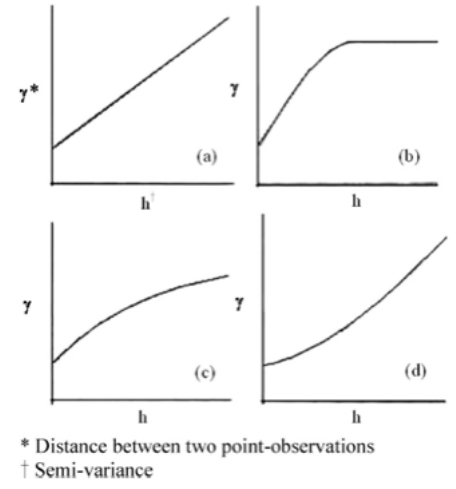
\includegraphics[width=10cm]{semivariogram-models.png}
\end{figure} 

There are a number of key points on the figures:

\begin{itemize}
    \item Range
    \begin{itemize}
        \item The Range is the point at which the semivariance first levels off
        \item Items within the range are autocorrelated (distance matters)
        \item Items outside the range are not autocorrelated (distance no longer changes the semivariance)
    \end{itemize}
    \item Sill 
    \begin{itemize}
        \item The Sill is the height at which the semivariance levels off to
    \end{itemize}
    \item Nugget
    \begin{itemize}
        \item The minimum value of semivariance ($\gamma (h = 0)$)
        \item Theoretically there is no semivariance when $h=0$, but in reality it is present due to measurement error or spatial sources of variation at distances smaller than the sample interval (or both)
    \end{itemize}
    \item Partial Sill
    \begin{itemize}
        \item Amount of semivariance between Sill and the Nugget
    \end{itemize}
\end{itemize}

\subsubsection{Predictions}

Now a model has been fit to the semivariance and autocorrelation can be observed, predictions can be made within the domain.
Kriging differs from IDW as it uses the semivariogram to calculate the weights.
There are a number of methods used in kriging:

\begin{enumerate}
    \item Ordinary kriging
    \begin{itemize}
        \item Assumes the constant mean is unknown
    \end{itemize}
    \item Universal kriging
    \begin{itemize}
        \item Assumes there's a prevailing trend, relaxing the assumption of stationarity for the mean, but maintaining a constant variance
        \item Trend is modelled with polynomial function, and subtracted from observed
        \item Semivariogram is modelled on the residuals to produce autocorrelations
    \end{itemize}
    \item Block kriging
    \begin{itemize}
        \item Estimates averaged values over gridded “blocks” rather than single points
        \item These blocks often have smaller prediction errors than are seen for individual points
    \end{itemize}
    \item Covariate kriging
    \begin{itemize}
        \item Additional observed variables (which are often correlated with each other and the variable of interest) are used to enhance the precision of the interpolation of the variable of interest at each location
    \end{itemize}
    \item Poisson kriging
    \begin{itemize}
        \item Used for incidence counts and disease rates 
    \end{itemize}
\end{enumerate}

\subsection{Limitations}

\begin{center}
    \fbox{Information for limitations from \href{https://www.publichealth.columbia.edu/research/population-health-methods/kriging-interpolation}{Columbia}}    
\end{center}

There are a number of limitations of kriging.

\begin{enumerate}
    \item Since the weights of the kriging interpolator depend on the modeled variogram, kriging is quite sensitive to mis-specification of the variogram model
    \item Similarly, the assumptions of the kriging model (e.g. that of second-order stationarity) may be difficult to meet in the context of many environmental exposures
    \begin{itemize}
        \item Some newer methods (e.g. Bayesian approaches) have thus been developed to try and surmount these obstacles
    \end{itemize}
    \item In general, the accuracy of interpolation by kriging will be limited if the number of sampled observations is small, the data is limited in spatial scope, or the data are in fact not amply spatially correlated
    \begin{itemize}
        \item In these cases, a sample variogram is hard to generate, and methods such as land-use regression may prove preferable to kriging for spatial prediction
    \end{itemize}
\end{enumerate}



\section{Natural Neighbour}

Natural neighbour is a local method that examines samples near the point of interest and evaluates the relative overlap with their areas.
The relative overlaps are then used to create the weights for interpolation.
Because of this, it is also known as "area-stealing" (Sibson) interpolation.
Natural neighbour interpolation therefore does not infer trends that are not already present in the data, and the surface passes through the points, and is smooth in between.

The areas are called Voronoi (Thiessen) polygons.
Voronoi polygons are created by examining the space around points and drawing the boundary so that every place inside the boundary is closest to the polygon's point than any other.
Formally this is written as:

\[R_{k} = \left\{x \in X \mid d(x, P_{k}) < d(x, P_{j}),  \text{ } \forall j \neq k)\right\}\]

\begin{conditions}
    R_{k} & Voronoi polygon of point $k$ \\
    P_{k} & Point $k$ \\ 
    P_{j} & Neighbouring point $j$
\end{conditions}

An example of this can be seen in the figure below.

\begin{figure}[h]
    \centering
    \label{Natural neighbour method of interpolation}
    \caption{Natural neighbour method of interpolation}
    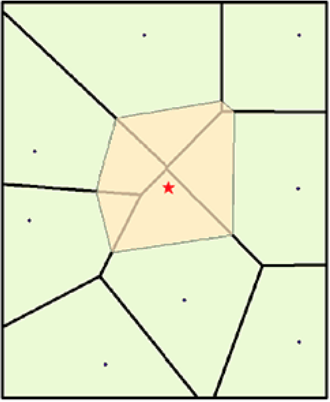
\includegraphics[width=5cm]{natural-neighbour.png}
\end{figure}

\section{Splines}

Splines are a smoothing function that pass through all the input points and attempt to create a smooth surface between them.
As such, it is best for gently varying surfaces e.g. pollution concentrations.
The surface is fit to a specified number of neighbouring input points.
The basic spline is also known as a thin plate interpolation.
There are two conditions that minimum curvature splines must follow:

\begin{enumerate}
    \item The surface must pass through all data points
    \item The surface must have minimum curvature i.e. minimize the cumulative sum of squares of the second derivative terms of the surface at each point
\end{enumerate}

One possible issue with thin plate interpolation is that there may be rapid change in first derivatives around each data point.
Increasing the number of points used for interpolation can help to smooth the surface as the cell is influenced by a greater number of more distant points.
Splines create rectangular regions of equal size, with the same number in the $x-$ and $y-$ directions.
Each region must contain at least 8 points, but different densities resulting from data that is not uniformly distributed can lead to regions containing different numbers of points.

Generally, the spline formula is:

\[S(x, y) = T(x, y) + \sum_{j=1}^{N} \lambda_{j} R(r_{j})\]

\begin{conditions}
    N & total number of points to be used in interpolation \\
    \lambda_{j} & coefficients found by the solution of a system of linear equations \\
    r_{j} & the distance from the point $(x,y)$ to the $j$th point
\end{conditions}

There are two spline types, which define the terms $T(x, y)$ and $R(r_{j})$ differently.

\subsection{Regularized splines}

A regularized spline creates a smooth and gradually changing surface, allowing values outside those observed in the data.

\[T(x, y) = a_{1} + a_{2}x + a_{3}y\]

\begin{conditions}
    a_{i} & coefficients found by the solutions of a system of linear equations
\end{conditions}

and, 

\[R(r) = \frac{1}{2 \pi} \left\{\frac{r^2}{4}\left[\ln \left(\frac{r}{2 \uptau}\right) + c - 1 \right] + \uptau^2\left[K_0 \left(\frac{r}{\uptau}\right) + c + \ln \left(\frac{r}{2 \pi}\right)\right]\right\}\]

\begin{conditions}
    r & the distance between the point and the sample \\
    \uptau^2 & the Weight parameter \\
    K_0 & the modified Bessel function \\
    c & a constant equal to 0.577215
\end{conditions}

In regularized splines, the Weight parameter ($\uptau^2$) specifies the weights attached to the third derivatives terms during minimization.
Larger weights result in smoother surfaces and smooth first-derivative surfaces.
Typical values range between 0 and 0.5.

\subsection{Tension splines}

A tension spline creates a less smooth surface with values more tightly constrained by the sample data range.

\[T(x, y) = a_{1} \]

\begin{conditions}
    a_{1} & a coefficient found by the solutions of a system of linear equations
\end{conditions}

and, 

\[R(r) = - \frac{1}{2 \pi \varphi^2} \left[\ln\left(\frac{r \varphi}{2}\right) + c + K_0 \left(r \varphi\right)\right]\]

\begin{conditions}
    r & the distance between the point and the sample \\
    \varphi^2 & the Weight parameter \\
    K_0 & the modified Bessel function \\
    c & a constant equal to 0.577215
\end{conditions}

The tension method differs from regularized splines as it attaches the Weight parameter ($\varphi^2$) to first-derivative terms, not third-derivative terms.
Larger values of $\varphi^2$  lower the tension and result in a coarser surface as the first-derivative surface is not smooth, passing through all the points.
$\varphi^2 = 0$ results in a basic thin plate surface.
Typical values range between 0 and 10.

\end{document}